\RequirePackage{filecontents}
\begin{filecontents*}{bib_Lec1.bib}

@book{chiang2005,
  title={Fundamental Methods of Mathematical Economics},
  author={Chiang, A.C. and Wainwright, K.},
  isbn={9780070109100},
  lccn={2004059546},
  series={Fourth edition},
  url={https://books.google.ca/books?id=LKIwAQAAMAAJ},
  year={2005},
  publisher={McGraw-Hill Education}
}
\end{filecontents*}

\documentclass[12pt]{article}
\usepackage{amsmath, amssymb, geometry}
\usepackage[most]{tcolorbox}
\geometry{margin=1in}

\usepackage{amsthm}
\usepackage{tikz}
\usepackage{pgfplots}
%\pgfplotsset{compat=1.18}



\title{Review of Sets and Functions}



\author{Muhebullah Karimzada}
\date{Fall 2025}

\tcbset{
  sectionbox/.style={
    colback=blue!10!white,
    colframe=blue!50!black,
    boxrule=0.8pt,
    arc=4pt,
    left=3pt,
    right=3pt,
    top=3pt,
    bottom=3pt
  },
  examplebox/.style={
    colback=green!10!white,
    colframe=green!50!black,
    boxrule=0.8pt,
    arc=4pt,
    left=3pt,
    right=3pt,
    top=3pt,
    bottom=3pt
  }
}

\begin{document}

\maketitle

\begin{center}
\begin{Large}
\textbf{ECON 320 - Introduction to Mathematical Economics}
\end{Large}
\end{center}
\newpage

% -------------------------------
% Section 1: Mathematical Models
% -------------------------------
\section*{A. Ingredients of a Mathematical Model}
\begin{tcolorbox}[sectionbox]
A mathematical model is a representation of an economic system using variables, equations, and assumptions to describe relationships and predict behavior.
\end{tcolorbox}

\begin{tcolorbox}[sectionbox]
\textbf{Ingredients:}
\begin{itemize}
    \item Variables and Equations
    \item Functional Relationships
    \item Assumptions
    \item Parameters
    \item Boundary Conditions
    \item Objectives
    \item Constraints
    \item Equilibrium Conditions
\end{itemize}
\end{tcolorbox}



\begin{tcolorbox}[sectionbox]
\textbf{1. Equations and Variables}\\
Equations represent economic relationships and show how variables interact.
\end{tcolorbox}

\begin{tcolorbox}[examplebox]
\textbf{Example:} Demand equation
\[
Q_d = 100 - 2P
\]
where $Q_d$ is quantity demanded and $P$ is price.
\end{tcolorbox}

\begin{tcolorbox}[sectionbox]
\textbf{2. Functional Relationships}\\
Functions describe how one variable depends on others. Can be linear, nonlinear, or multi-variable.
\end{tcolorbox}

\begin{tcolorbox}[examplebox]
\textbf{Example:} Cobb-Douglas production function
\[
Y = A L^\alpha K^\beta
\]
where $Y$ is output, $L$ is labor, $K$ is capital, and $A$, $\alpha$, $\beta$ are constants.
\end{tcolorbox}

\begin{tcolorbox}[sectionbox]
\textbf{3. Assumptions}\\
Simplify reality for tractability, e.g., rational behavior, perfect competition, or ceteris paribus.
\end{tcolorbox}

\begin{tcolorbox}[examplebox]
\textbf{Example:} Perfect competition implies no single buyer/seller can influence market price.
\end{tcolorbox}

\begin{tcolorbox}[sectionbox]
\textbf{4. Parameters}\\
Constants defining relationships, estimated from data.
\end{tcolorbox}

\begin{tcolorbox}[examplebox]
\textbf{Example:} In $Q_d = 100 - 2P$, the slope $-2$ is a parameter showing sensitivity of demand to price.
\end{tcolorbox}

\begin{tcolorbox}[sectionbox]
\textbf{5. Boundary Conditions}\\
Initial or boundary values required for solving models, especially differential equations.
\end{tcolorbox}

\begin{tcolorbox}[examplebox]
\textbf{Example:} Capital accumulation model with $K(0) = K_0$ as initial condition.
\end{tcolorbox}

\begin{tcolorbox}[sectionbox]
\textbf{6. Objectives}\\
Models often optimize objectives like profit, utility, or cost.
\end{tcolorbox}

\begin{tcolorbox}[examplebox]
\textbf{Example:} Profit maximization:
\[
\pi = P \cdot Q - C(Q)
\]
where $P$ is price, $Q$ is quantity, $C(Q)$ is cost.
\end{tcolorbox}

\begin{tcolorbox}[sectionbox]
\textbf{7. Constraints}\\
Limitations like resources, budget, or technology.
\end{tcolorbox}

\begin{tcolorbox}[examplebox]
\textbf{Example:} Budget constraint:
\[
P_x \cdot x + P_y \cdot y = I
\]
where $P_x$, $P_y$ are prices and $I$ is income.
\end{tcolorbox}

\begin{tcolorbox}[sectionbox]
\textbf{8. Equilibrium Conditions}\\
States where economic forces balance, e.g., supply equals demand.
\end{tcolorbox}

\begin{tcolorbox}[examplebox]
\textbf{Example:} Market equilibrium:
\[
Q_s = Q_d
\]
\end{tcolorbox}

\begin{tcolorbox}[sectionbox]
\textbf{Conclusion}\\
Mathematical models integrate these ingredients to analyze and predict economic behavior systematically.
\end{tcolorbox}
% -------------------------------
% Section 2: Real Numbers
% -------------------------------
\section*{B. Real Number System}

\begin{tcolorbox}[sectionbox]

The real number system is the foundation of mathematical analysis in economics. It includes both rational numbers (fractions) and irrational numbers (non-repeating, non-terminating decimals).
\end{tcolorbox}

\begin{tcolorbox}[sectionbox]
\textbf{1.  Classification of Numbers}
\begin{itemize}
    \item \textbf{Natural Numbers ($\mathbb{N}$):} $1,2,3,\dots$ 
    \item \textbf{Whole Numbers ($\mathbb{W}$):} $0,1,2,3,\dots$
    \item \textbf{Integers ($\mathbb{Z}$):} $\dots,-2,-1,0,1,2,\dots$
    \item \textbf{Rational Numbers ($\mathbb{Q}$):} numbers expressible as $\frac{p}{q}$, $q\neq0$; e.g., $\frac{2}{3},0.75$
    \item \textbf{Irrational Numbers:} cannot be expressed as fractions; e.g., $\pi,\sqrt{2}$
    \item \textbf{Real Numbers ($\mathbb{R}$):} $\mathbb{R} = \mathbb{Q} \cup$ (irrationals)
\end{itemize}
\end{tcolorbox}

\begin{tcolorbox}[sectionbox]
\textbf{2. Properties of Real Numbers}
\begin{itemize}
    \item \textbf{Algebraic:} closure, commutative, associative, distributive laws

    \item \textbf{Completeness:} every non-empty set bounded above has a least upper bound
\end{itemize}
\end{tcolorbox}

\begin{tcolorbox}[examplebox]
\textbf{Example of Completeness:} The set $\{x \in \mathbb{Q} \mid x^2 < 2\}$ has no rational supremum, but its supremum in $\mathbb{R}$ is $\sqrt{2}$.
\end{tcolorbox}

\begin{tcolorbox}[sectionbox]
\textbf{3. Intervals of Real Numbers}
\begin{itemize}
    \item \textbf{Closed Interval:} $[a,b] = \{x \in \mathbb{R} \mid a \le x \le b\}$
    \item \textbf{Open Interval:} $(a,b) = \{x \in \mathbb{R} \mid a < x < b\}$
    \item \textbf{Half-Open:} $[a,b)$ or $(a,b]$
\end{itemize}
\end{tcolorbox}

\begin{tcolorbox}[sectionbox]
\textbf{4. Absolute Value}
\[
|x| = 
\begin{cases} 
x & \text{if } x \ge 0 \\ 
-x & \text{if } x < 0
\end{cases}
\]
Properties:
\begin{itemize}
    \item $|xy| = |x||y|$
    \item $|x+y| \le |x| + |y|$ (Triangle inequality)
\end{itemize}
\end{tcolorbox}

\begin{tcolorbox}[sectionbox]
\textbf{5. Representation on the Number Line}\\
Real numbers are points on a continuous line. Distance between $a$ and $b$ is $|a-b|$.
\end{tcolorbox}

\begin{tcolorbox}[sectionbox]
\textbf{6. Applications in Economics}\\
Real numbers allow modeling continuous variables: prices, quantities, interest rates, output. They are essential for derivatives, integrals, and continuous functions.
\end{tcolorbox}

\begin{tcolorbox}[examplebox]
\textbf{Examples of Real Numbers:}
\begin{itemize}
    \item Integers: $0,7,-3$
    \item Rational: $\frac{5}{2},-0.4$
    \item Irrational: $\pi, \sqrt{3}$
    \item All belong to $\mathbb{R}$
\end{itemize}
\end{tcolorbox}

\begin{tcolorbox}[sectionbox]

Understanding the real number system is fundamental for mathematical modeling in economics and provides the basis for analysis of continuous variables and functions.
\end{tcolorbox}



% -------------------------------
% Section 3: Sets
% -------------------------------
\section*{C. The Concept of Sets}
\begin{tcolorbox}[sectionbox]
A set is a collection of objects called elements. Sets are foundational for grouping and modeling in economics.
\end{tcolorbox}


\begin{tcolorbox}[sectionbox]
\textbf{1. Elements of a Set}\\
- Objects contained in a set are called elements.\\
- Notation: $x \in A$ means $x$ is in set $A$; $y \notin A$ means $y$ is not in $A$.
\end{tcolorbox}

\begin{tcolorbox}[examplebox]
\textbf{Example:} 
\[
A = \{apple, banana, orange\}, \quad apple \in A, \quad mango \notin A
\]
\end{tcolorbox}

\begin{tcolorbox}[sectionbox]
\textbf{2. Types of Sets}
\begin{itemize}
    \item \textbf{Finite Set:} Limited number of elements, e.g., $A=\{1,2,3\}$
    \item \textbf{Infinite Set:} Elements are unbounded, e.g., $B=\{1,2,3,\dots\}$
    \item \textbf{Empty Set:} Contains no elements, $\emptyset$ or $\{\}$
    \item \textbf{Singleton Set:} Contains exactly one element, $S=\{0\}$
    \item \textbf{Subsets:} $A \subseteq B$ means all elements of $A$ are in $B$
    \item \textbf{Universal Set:} $U$ contains all elements under consideration
\end{itemize}
\end{tcolorbox}

\begin{tcolorbox}[sectionbox]
\textbf{3. Set Operations}
\begin{itemize}
    \item \textbf{Union ($\cup$):} $A \cup B = \{x \mid x \in A \text{ or } x \in B\}$
    \item \textbf{Intersection ($\cap$):} $A \cap B = \{x \mid x \in A \text{ and } x \in B\}$
    \item \textbf{Difference ($\setminus$):} $A \setminus B = \{x \mid x \in A, x \notin B\}$
    \item \textbf{Complement:} $A^c = U \setminus A$
    \item \textbf{Cartesian Product:} $A \times B = \{(a,b) \mid a \in A, b \in B\}$
\end{itemize}
\end{tcolorbox}

\begin{tcolorbox}[examplebox]
\textbf{Example:} Let $A=\{1,2\}, B=\{2,3\}$, $U=\{1,2,3,4\}$
\begin{itemize}
    \item $A \cup B = \{1,2,3\}$
    \item $A \cap B = \{2\}$
    \item $A \setminus B = \{1\}$
    \item $A^c = \{3,4\}$
    \item $A \times B = \{(1,2),(1,3),(2,2),(2,3)\}$
\end{itemize}
\end{tcolorbox}

\begin{tcolorbox}[sectionbox]
\textbf{4. Venn Diagrams}\\
A visual representation of sets and their relationships. Useful for unions, intersections, complements, and illustrating market overlaps, population segments, or preferences.

Let $A$ and $B$ be two sets. The following diagrams illustrate the fundamental set operations.  

%========================
% A union B
%========================
\subsection*{$A \cup B$ (Union)}
\textbf{Definition:} The union of two sets $A$ and $B$ is the set of all elements that are in $A$, in $B$, or in both.  

\begin{center}
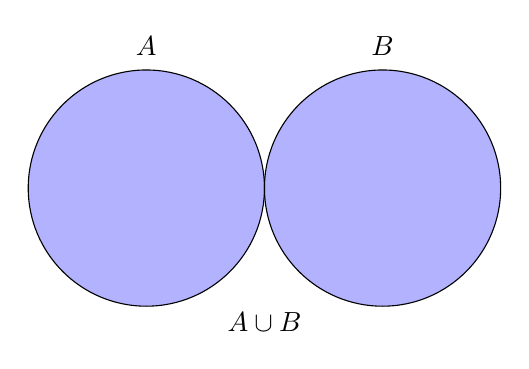
\begin{tikzpicture}
% Fill union
\begin{scope}
  \clip (0,0) circle (1.5cm);

\end{scope}
\fill[blue!30] (0,0) circle (1.5cm);
  \fill[blue!30] (3,0) circle (1.5cm);
% Circles
\draw (0,0) circle (1.5cm);
\draw (3,0) circle (1.5cm);

% Labels
\node at (0,1.8) {$A$};
\node at (3,1.8) {$B$};
\node at (1.5,-1.7) {$A \cup B$};
\end{tikzpicture}
\end{center}

\textbf{Explanation:} All elements that belong to either $A$, $B$, or both are included. The entire area covered by both circles is shaded.

%========================
% A intersection B
%========================
\subsection*{$A \cap B$ (Intersection)}
\textbf{Definition:} The intersection of $A$ and $B$ is the set of elements that are in both $A$ and $B$.  

\begin{center}
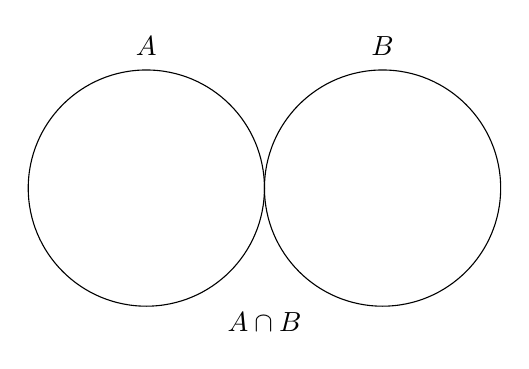
\begin{tikzpicture}
% Fill intersection
\begin{scope}
  \clip (0,0) circle (1.5cm);
  \fill[green!40] (3,0) circle (1.5cm);
\end{scope}

% Circles
\draw (0,0) circle (1.5cm);
\draw (3,0) circle (1.5cm);

% Labels
\node at (0,1.8) {$A$};
\node at (3,1.8) {$B$};
\node at (1.5,-1.7) {$A \cap B$};
\end{tikzpicture}
\end{center}

\begin{center}
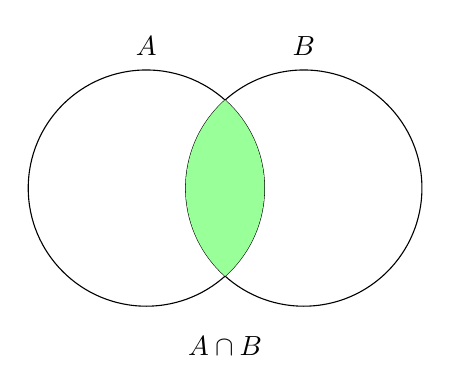
\begin{tikzpicture}
% Draw circles
\draw (0,0) circle (1.5cm);
\draw (2,0) circle (1.5cm);

% Shade intersection only
\begin{scope}
  \clip (0,0) circle (1.5cm);
  \fill[green!40] (2,0) circle (1.5cm);
\end{scope}

% Labels
\node at (0,1.8) {$A$};
\node at (2,1.8) {$B$};
\node at (1,-2) {$A \cap B$};
\end{tikzpicture}
\end{center}

\textbf{Explanation:} Only elements that belong to \textbf{both} sets are included. The overlapping area is shaded.


\end{tcolorbox}


\begin{tcolorbox}[sectionbox]

%========================
% A minus B
%========================
\subsection*{$A - B$ (Difference)}
\textbf{Definition:} The difference $A - B$ is the set of elements that are in $A$ but not in $B$.  

\begin{center}
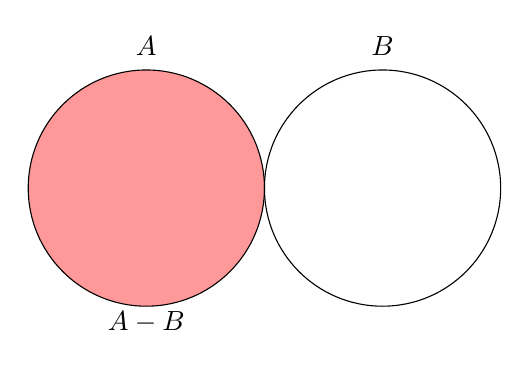
\begin{tikzpicture}
% Fill A only
\fill[red!40] (0,0) circle (1.5cm);
\begin{scope}
  \clip (3,0) circle (1.5cm);
  \fill[white] (0,0) circle (1.5cm);
\end{scope}

% Circles
\draw (0,0) circle (1.5cm);
\draw (3,0) circle (1.5cm);

% Labels
\node at (0,1.8) {$A$};
\node at (3,1.8) {$B$};
\node at (0,-1.7) {$A - B$};
\end{tikzpicture}
\end{center}

\textbf{Explanation:} Elements unique to $A$ are included; the overlapping region with $B$ is excluded.

%========================
% B minus A
%========================
\subsection*{$B - A$ (Difference)}
\textbf{Definition:} The difference $B - A$ is the set of elements that are in $B$ but not in $A$.  

\begin{center}
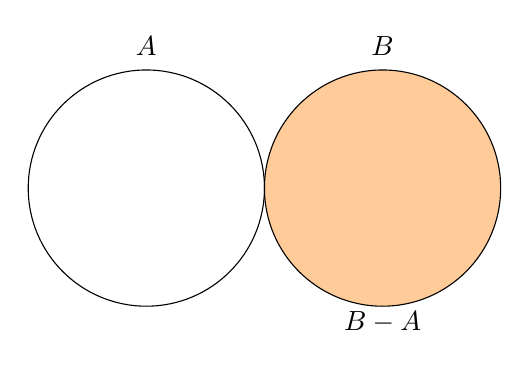
\begin{tikzpicture}
% Fill B only
\fill[orange!40] (3,0) circle (1.5cm);
\begin{scope}
  \clip (0,0) circle (1.5cm);
  \fill[white] (3,0) circle (1.5cm);
\end{scope}

% Circles
\draw (0,0) circle (1.5cm);
\draw (3,0) circle (1.5cm);

% Labels
\node at (0,1.8) {$A$};
\node at (3,1.8) {$B$};
\node at (3,-1.7) {$B - A$};
\end{tikzpicture}
\end{center}

\textbf{Explanation:} Elements unique to $B$ are included; overlapping with $A$ is excluded.

%========================
% Complement of A
%========================
\subsection*{$A^c$ (Complement)}
\textbf{Definition:} The complement of $A$, denoted $A^c$, is the set of all elements not in $A$.  

\begin{center}
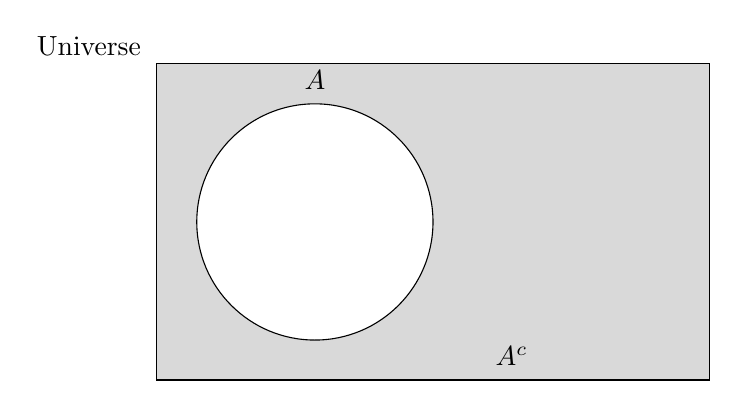
\begin{tikzpicture}
% Draw universe rectangle
\draw[thick] (-2,-2) rectangle (5,2);
\node at (-2.1,3,2) {Universe};

% Fill complement
\fill[gray!30] (-2,-2) rectangle (5,2);
\fill[white] (0,0) circle (1.5cm);

% Draw A
\draw (0,0) circle (1.5cm);
\node at (0,1.8) {$A$};
\node at (2.5,-1.7) {$A^c$};
\end{tikzpicture}
\end{center}

\textbf{Explanation:} The shaded area represents all elements \textbf{outside} set $A$, i.e., everything in the universe except $A$.
\end{tcolorbox}

\begin{tcolorbox}[sectionbox]
\textbf{5. Properties of Set Operations}
\begin{itemize}
    \item \textbf{Commutative:} $A \cup B = B \cup A$, $A \cap B = B \cap A$
    \item \textbf{Associative:} $(A \cup B) \cup C = A \cup (B \cup C)$
    \item \textbf{Distributive:} $A \cap (B \cup C) = (A \cap B) \cup (A \cap C)$
    \item \textbf{De Morgan’s Laws:} $(A \cup B)^c = A^c \cap B^c$, $(A \cap B)^c = A^c \cup B^c$
\end{itemize}
\end{tcolorbox}

\begin{tcolorbox}[sectionbox]
\textbf{6. Applications in Economics}
\begin{itemize}
    \item Consumer choice: set of all goods consumed
    \item Production: set of feasible production combinations
    \item Market analysis: set of firms, buyers, or products
    \item Probability and uncertainty: events as subsets of sample space
\end{itemize}
\end{tcolorbox}

\begin{tcolorbox}[sectionbox]

The concept of sets provides a fundamental framework for grouping elements, performing operations, and modeling economic phenomena systematically.
\end{tcolorbox}

% -------------------------------
% Section 4: Relations
% -------------------------------
\section*{D. Relations and Functions}
% -------------------------------
% Section 1: Introduction
% -------------------------------

\begin{tcolorbox}[sectionbox]
Relations and functions are fundamental concepts that describe how elements from one set are associated with elements of another. They are widely used in economics to model demand, supply, production, and preferences.
\end{tcolorbox}

% -------------------------------
% Section 2: Relations
% -------------------------------
\section*{1. Relations}

\begin{tcolorbox}[sectionbox]
\textbf{Definition:} A relation $R$ from set $A$ to set $B$ is a subset of the Cartesian product $A \times B$:
\[
R \subseteq A \times B
\]
Notation: If $(a,b) \in R$, we write $a \, R \, b$.
\end{tcolorbox}

\begin{tcolorbox}[examplebox]
\textbf{Example:} Let $A = \{1,2,3\}$, $B = \{x,y\}$  
Relation $R = \{(1,x),(2,y),(3,x)\}$
\end{tcolorbox}

\begin{tcolorbox}[sectionbox]
\textbf{Types of Relations:}
\begin{itemize}
    \item Reflexive: $a R a$ for all $a \in A$
    \item Symmetric: If $a R b$, then $b R a$
    \item Transitive: If $a R b$ and $b R c$, then $a R c$
    \item Equivalence Relation: Reflexive, symmetric, and transitive
    \item Partial Order: Reflexive, antisymmetric, and transitive (e.g., $\le$)
\end{itemize}
\end{tcolorbox}

\begin{tcolorbox}[examplebox]
\textbf{Economic Example:} Preference relation $\succeq$ on consumption bundles: $(x_1,x_2) \in R$ if $x_1$ is at least as preferred as $x_2$.
\end{tcolorbox}

% -------------------------------
% Section 3: Functions
% -------------------------------
\section*{2. Functions}

\begin{tcolorbox}[sectionbox]
A function $f$ from set $A$ (domain) to set $B$ (codomain) is a relation where each element of $A$ is related to exactly one element of $B$:
\[
f: A \to B, \quad f(a) = b
\]
\end{tcolorbox}

\begin{tcolorbox}[examplebox]
\textbf{Examples:}
\begin{itemize}
    \item $f(x) = 2x + 3, \quad x \in \mathbb{R}$
    \item Demand function: $Q_d(P) = 100 - 2P$
    \item Production function: $Y = F(K,L)$
\end{itemize}
\end{tcolorbox}


\begin{tcolorbox}[sectionbox]
\textbf{Properties of Functions:}
\begin{itemize}
    \item Domain: input values
    \item Codomain: potential output values
    \item Range (Image): actual output values
    \item Monotonicity: increasing or decreasing
    \item Continuity: no abrupt jumps
    \item Differentiability: smooth changes
\end{itemize}
\end{tcolorbox}

\begin{tcolorbox}[examplebox]
\textbf{Examples:}
\begin{itemize}
    \item $f(x) = x^2, x \in \mathbb{R}$, Range: $[0,\infty)$
    \item Production function: $Y = K^{0.3} L^{0.7}, K,L \ge 0$
\end{itemize}
\end{tcolorbox}

\begin{tcolorbox}[sectionbox]
\textbf{Classification of Functions:}

\textbf{2.1 According to Number of Variables:}
\begin{itemize}
    \item \textbf{Single-variable:} $y = f(x)$, e.g., $Q_d(P) = 100 - 2P$
    \item \textbf{Multivariable:} $z = f(x_1, x_2, \dots, x_n)$, e.g., $Y = F(K,L)$
\end{itemize}

%\textbf{2.2 According to Mapping Properties:}
%\begin{itemize}
 %   \item \textbf{Injective (One-to-One):} Each domain element maps to a unique codomain element, e.g., $f(x)=2x+3$
 %   \item \textbf{Surjective (Onto):} Every codomain element has a pre-image, e.g., $f(x)=x^3$
   % \item \textbf{Bijective:} Both injective and surjective, e.g., $f(x)=x+5$
%\end{itemize}

\textbf{2.3 According to Continuity and Smoothness:}
\begin{itemize}
    \item \textbf{Continuous:} No jumps, e.g., $f(x)=x^2$
    \item \textbf{Discontinuous:} Has jumps, e.g., step functions
    \item \textbf{Differentiable:} Smooth, derivative exists, e.g., $f(x)=x^3$
    \item \textbf{Non-differentiable:} Sharp corners, e.g., $f(x)=|x|$ at $x=0$
\end{itemize}

\textbf{2.4 According to Nature of Function:}
\begin{itemize}
    \item \textbf{Linear:} $y = a + bx$, constant slope
    \item \textbf{Nonlinear:} $y = ax^2 + bx + c$, slope varies, e.g., Cobb-Douglas $Y = K^\alpha L^\beta$
    \item \textbf{Monotonic:} Increasing or decreasing
    \item \textbf{Homogeneous:} Scaling inputs scales output, e.g., $f(tK,tL)=t^r f(K,L)$
    \item \textbf{Explicit vs Implicit:} $y=f(x)$ (explicit), $F(x,y)=0$ (implicit)
\end{itemize}
\end{tcolorbox}

\begin{tcolorbox}[sectionbox]
\textbf{2.5 According to Output Mapping:}
\begin{itemize}
    \item \textbf{Real-Valued:} $f:\mathbb{R}^n \to \mathbb{R}$, e.g., $U(x_1,x_2)=x_1^{0.5}x_2^{0.5}$
    \item \textbf{Vector-Valued:} $f:\mathbb{R}^n \to \mathbb{R}^m$, e.g., market equilibrium mapping
    \item \textbf{Boolean:} Maps to 0 or 1, e.g., indicator functions
\end{itemize}



\textbf{2.6 Special Functions in Economics:}
Step functions, piecewise functions, quadratic/polynomial functions, exponential and logarithmic functions.
\end{tcolorbox}

\begin{tcolorbox}[sectionbox]
\textbf{Function Operations:}
\begin{itemize}
    \item Addition: $(f+g)(x) = f(x) + g(x)$
    \item Multiplication: $(f \cdot g)(x) = f(x) \cdot g(x)$
    \item Composition: $(f \circ g)(x) = f(g(x))$
\end{itemize}
\end{tcolorbox}

% -------------------------------
% Section 3: Summary Table
% -------------------------------
\section*{ Summary Table of Function Types}
\begin{tcolorbox}[examplebox]
\begin{tabular}{|l|l|l|}
\hline
\textbf{Type} & \textbf{Definition} & \textbf{Economic Example} \\
\hline
Linear & Constant slope & Linear demand $Q=a-bP$ \\
Nonlinear & Slope changes & Cobb-Douglas $Y=K^\alpha L^\beta$ \\
Monotonic & Increasing/decreasing & Utility in goods \\
Injective & Unique mapping & Price-to-demand mapping \\
Surjective & Covers codomain & Production mapping \\
Bijective & One-to-one & Resource allocation mapping \\
Continuous & No jumps & Smooth cost function \\
Differentiable & Derivative exists & Production optimization \\
Homogeneous & Scale property & Returns to scale in production \\
\hline
\end{tabular}
\end{tcolorbox}






\begin{tcolorbox}[sectionbox]
\textbf{Graphical Representation:}
\begin{itemize}
    \item Graph: set of points $(x,f(x))$
    \item Vertical line test: ensures each $x$ has exactly one $y$
\end{itemize}

A function maps each element of one set (domain) to exactly one element of another set (codomain).  

\[
f: X \to Y
\]

\textbf{Example 1: Demand Function}  
\[
q(p) = 100 - 2p
\]

\begin{center}
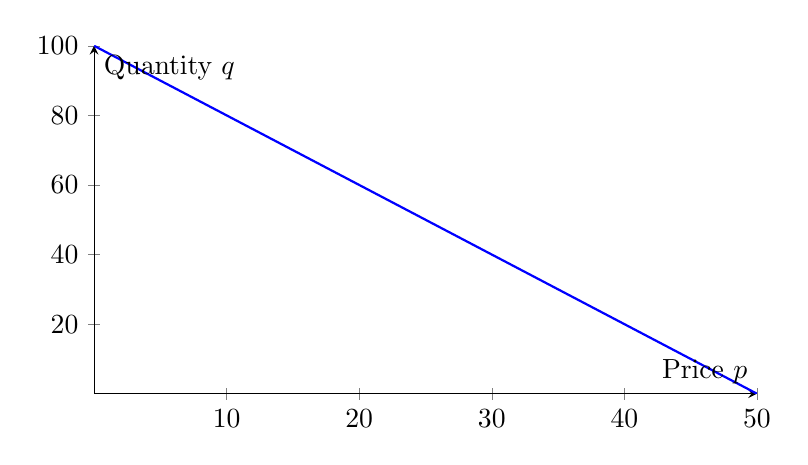
\begin{tikzpicture}
\begin{axis}[
    axis lines = middle,
    xlabel = {Price $p$},
    ylabel = {Quantity $q$},
    domain=0:50,
    samples=100,
    width=10cm,
    height=6cm
]
\addplot[blue, thick] {100 - 2*x};
\end{axis}
\end{tikzpicture}
\end{center}





\textbf{Example 2: Utility Function:} $U(x,y) = \sqrt{x}\sqrt{y}$ (Cobb–Douglas).  

\begin{center}
\begin{tikzpicture}
\begin{axis}[
    axis lines = middle,
    xlabel = {$x$ (good 1)},
    ylabel = {$y$ (good 2)},
    domain=0.1:10,
    samples=50,
    width=10cm,
    height=7cm
]
\addplot[red, thick] ({x},{36/(x)}); % Indifference curve U=6
\node at (axis cs:5,24) {$U=6$};
\end{axis}
\end{tikzpicture}
\end{center}
\end{tcolorbox}



\begin{tcolorbox}[sectionbox]

\textbf{Example 3: Production Function:} $Q(K,L) = K^{0.3} L^{0.7}$  
(isoquant for $Q=10$).  

\begin{center}
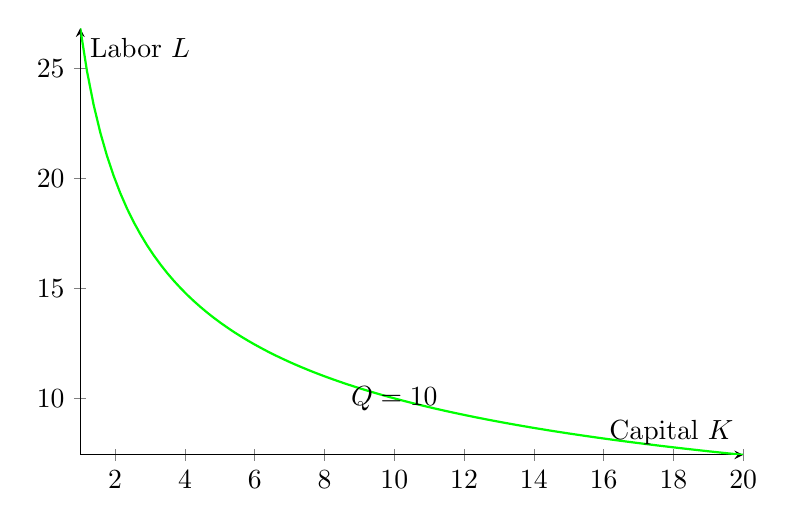
\begin{tikzpicture}
\begin{axis}[
    axis lines = middle,
    xlabel = {Capital $K$},
    ylabel = {Labor $L$},
    domain=1:20,
    samples=100,
    width=10cm,
    height=7cm
]
\addplot[green, thick] ({x},{(10/(x^0.3))^(1/0.7)});
\node at (axis cs:10,10) {$Q=10$};
\end{axis}
\end{tikzpicture}
\end{center}

\end{tcolorbox}



\begin{tcolorbox}[sectionbox]
\textbf{Applications in Economics:}
\begin{itemize}
    \item Consumer theory: Utility and demand functions
    \item Production theory: Production and cost functions
    \item Market analysis: Price-quantity mappings
    \item Growth models: Exponential/logarithmic growth
    \item Optimization: Monotonic and differentiable functions for maxima/minima
\end{itemize}
\end{tcolorbox}

\begin{tcolorbox}[sectionbox]
Functions and relations provide the mathematical framework for modeling economic relationships, linking variables systematically for analysis and prediction.
\end{tcolorbox}



\bigskip
\hrule
\bigskip


\bigskip

\begin{thebibliography}{9}
\bibitem{CW}
Chiang, A.\,C. and Wainwright, K.\ (2005). \emph{Fundamental Methods of Mathematical Economics}, 4th ed., McGraw--Hill.

\bibitem{SB}
Simon, C.\,P. and Blume, L.\ (2010). \emph{Mathematics for Economists}. W.\,W. Norton.

\bibitem{SH}
Syds\ae ter, K. and Hammond, P.\ (2022). \emph{Essential Mathematics for Economic Analysis}, 6th ed., Pearson.
\end{thebibliography}




\end{document}
